MINI-V(minitua vessel) was created in order to test the software easily in the Covid-19. Over the past several years, 
we couldn't conduct the experiment on the ocean or lake because of the COVID-19.
We were prohibited to meet and create the parts of WAM-V.
 In addition, the law about vessels is very strict.
So, we can't float the boat easily. The WAM-V is so big and it is hard work and costs too much to carry WAM-V to the lake. 
Then, we need a sustainable system to develop the automotive vessel.
As mentioned above, the simulator is used for developing navigation systems, and it doesn't need to use WAM-V.
The perception array was created to get the sensor data for software tests. They made it easier for us to develop software without ships.
 However, the software and hardware integration is the most important to conduct tasks. Then, MINI-V was created 
to make it easier to do the test and the integration.

The concepts of MINI-V are follows:
\begin{enumerate}
  \item easy assembly, transport, and experiment,
  \item open source software and hardware,
  \item high compatibility between WAM-V and MINI-V.
\end{enumerate}
MINI-V is created to be easy to carry, and we can carry them by suitcase like Fig. (b). 
It is also assembled simply. We develop this vessel on open source. So, other people can play or test their software with MINI-V. Finally,
we expect the high compatibility between WAM-V and MINI-V, and it will make it easy to migrate developed software on MINI-V toWAM-V. However, 
MINI-V have not had complete compatibility yet.
We have future tasks to create a little bigger vessel to have compatible hardware and software such as batteries and sensors, and so on.

\begin{figure}[t]
  \begin{center}
    \scalebox{0.24}{
      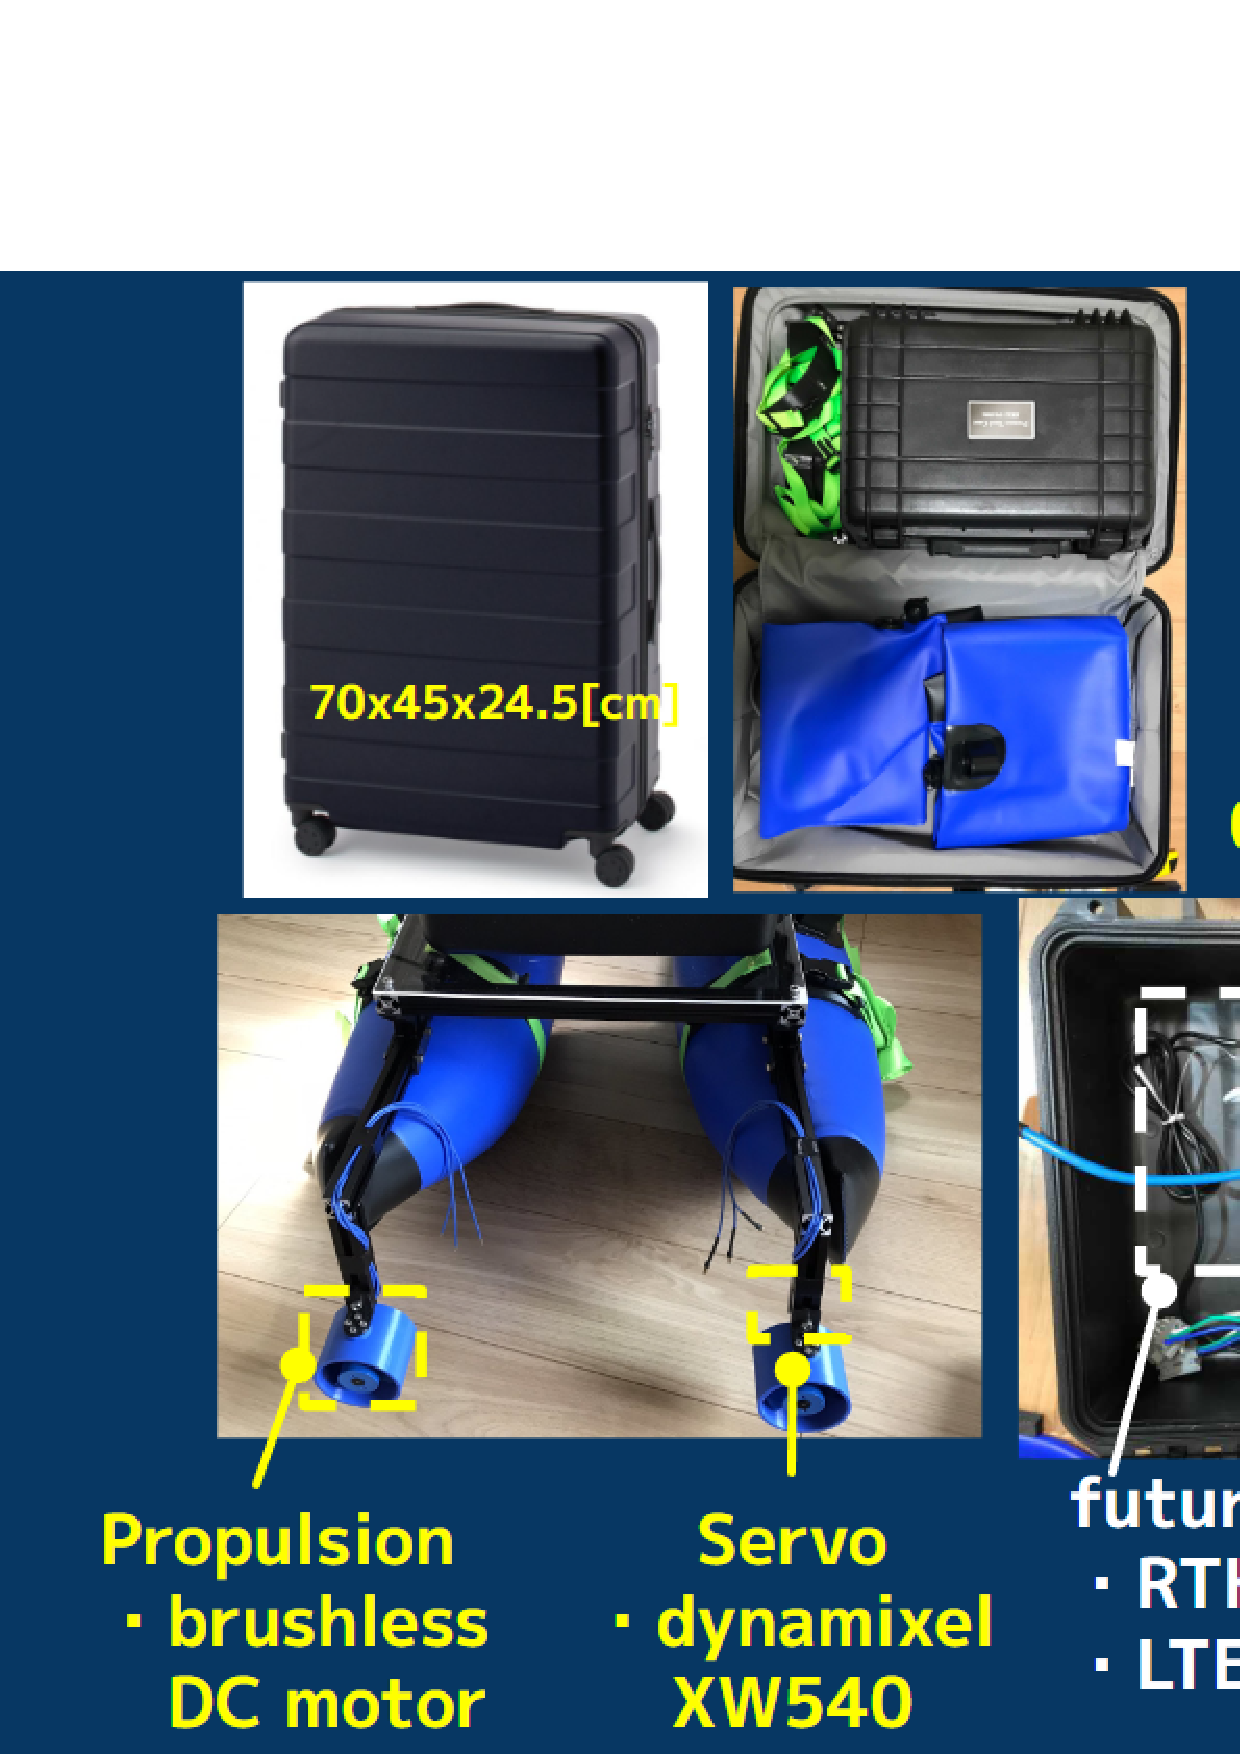
\includegraphics{figure/mini_v_component.png}
    }
    \caption{Hardware components of MINI-V}
  \end{center}
  \label{fig:mini_v}
\end{figure}